To check convergence we run the poisson solver with the load function and exact solution given in equation (\ref{loadfunc2}). We run the exact same configuration 11 times on Kongull with only $N$ changing each iteration. We let $n$ vary from $2^4$ to $2^{14}$. We run the job with 3 openMP threads and 12 MPI processors. The program returns the maximum error over the whole domain. This is then imported to matlab and plotted on the logarithm scale in figure \ref{fig:checkConv}. For the given test data we have quadratic convergence as expected.\\
\\
\begin{figure}[h]
\centering
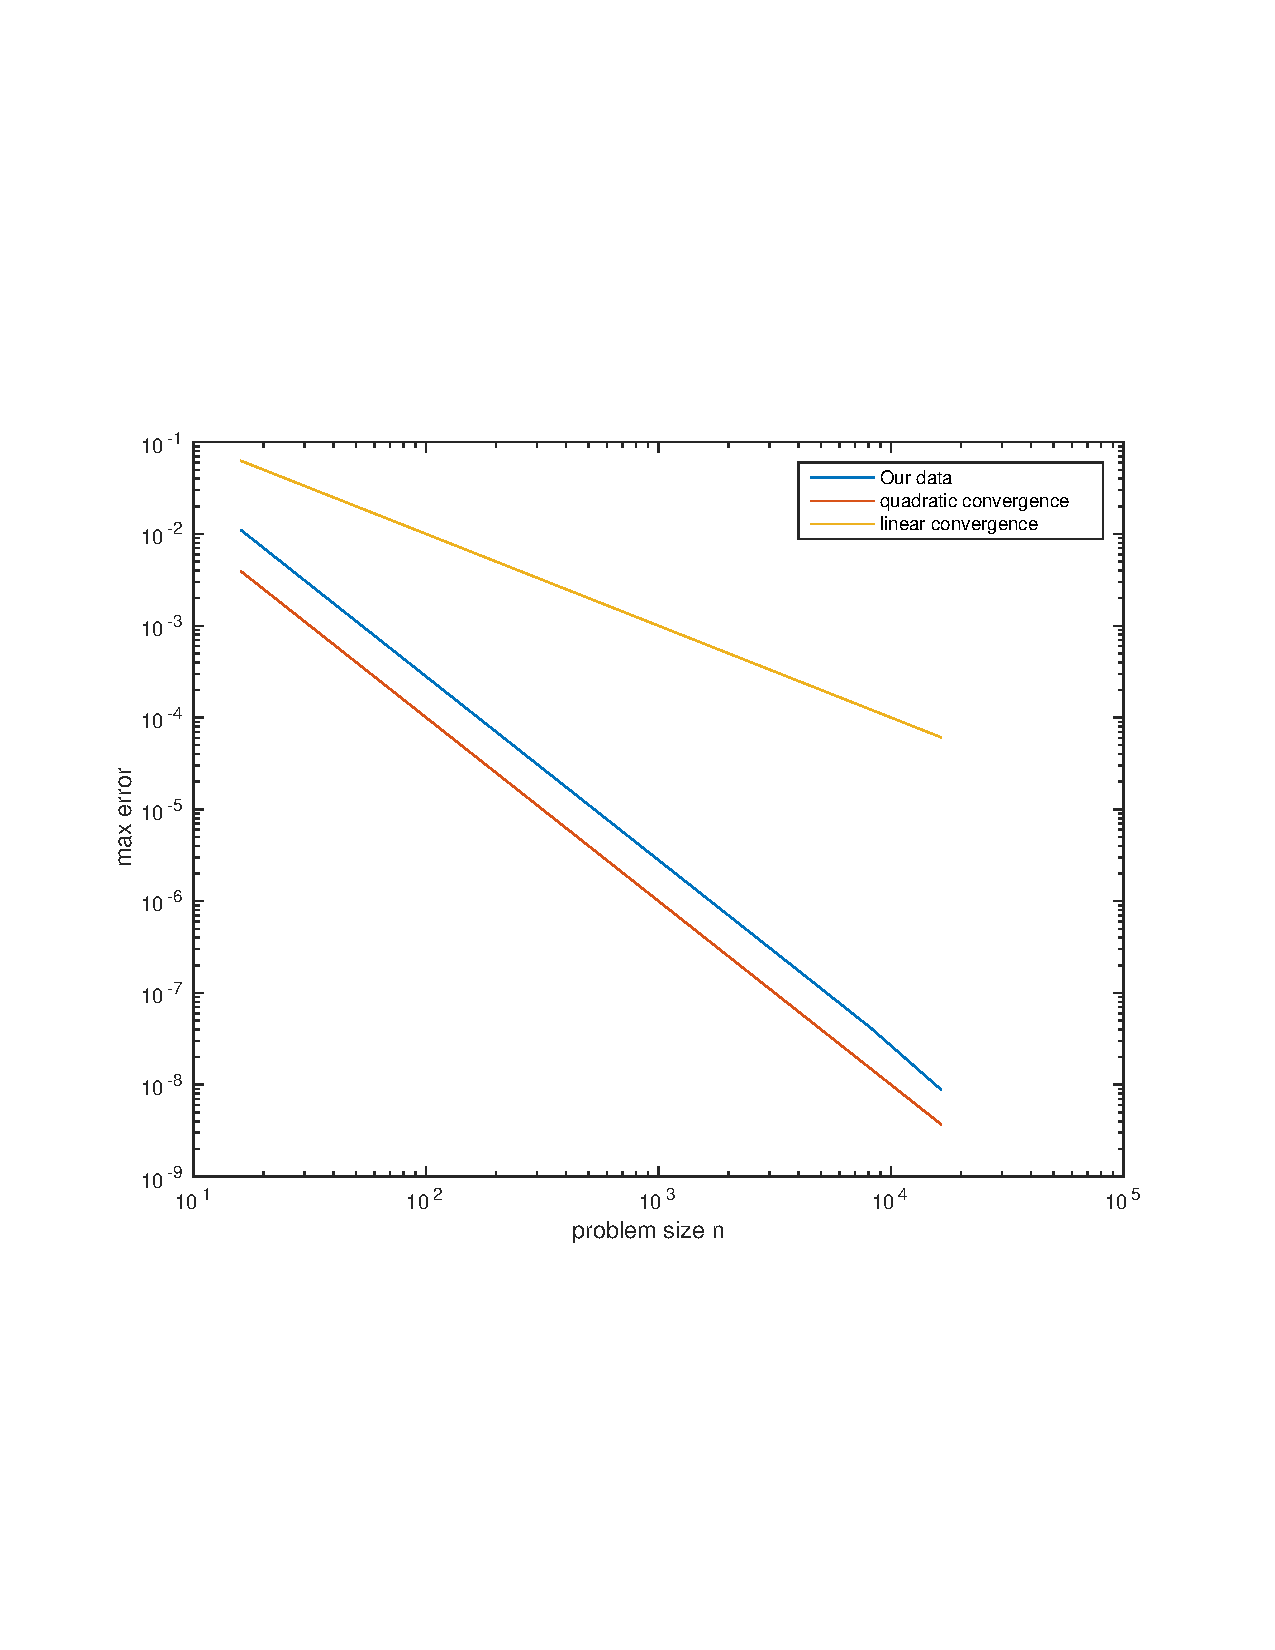
\includegraphics[width=0.6\linewidth]{./figures/checkConv}
\caption{Shows that the result from the convergence test compared with curves with slope $h$ and $h^2$. We see that our data has the same slope as $h^2$}
\label{fig:checkConv}
\end{figure}
The program was also tested with various configurations of $n, p$ and $t$ and seems to be working correctly for all of them.
